\section{Polynomial Decusping}

\section{Subplane Collision Probabilities}

\subsection{Subplane CMFD}

\subsection{Collision Probabilities Decusping}

\section{Subray Method of Characteristics}

\subsection{Motivation}

\subsubsection{1D MOC Code and Problem Description}

The code is set up to take in a description of pins and materials to be used for the calculations.  For the geometry, a pin pitch is specified which is used for all pins.  Each pin consists of a list of radii.  Assuming a square pin cell, these pins are then transformed from cylindrical geometry to slab geometry while preserving the volume fraction of each material.  Thus, the thickness of the pin slab is equal to the pin pitch, but the width of the fuel material will not be equal to input radius, since the volume fractions are preserved.  One material is then specified for each region, though each material region is divided into many sub-regions for the MOC calculations.  These materials are defined by a separate cross-section library file.  This file uses the ``user library'' format supported by MPACT, which allows the user to put in macroscopic cross-sections for absorption, nu-fission, kappa-fission, chi, and scattering moments.  For all these calculations, the C5G7 benchmark cross-sections \cite{EELewisC5G72003,EELewisC5G7extended2005} were used.  These cross sections are included in Appendix \ref{app:c5g7xs}.

For the MOC sweeps, a Gaussian quadrature \cite{HandbookOfMathFunctions1972} is used with 2, 4, 8, 16, or 32 polar angles, with half of the angles being used in each direction.  The MOC sweeps are done similarly to how they are done in MPACT, with the loop over energy groups being the innermost loop.  The code can be run as either a fixed source solver or an eigenvalue solver.  For the eigenvalue mode, power iteration is used after each MOC calculation to determine and updated k$_{eff}$.  The fixed source mode can be used to run either a specified number of iterations or to run until the scattering source is converged below some tolerance.  This allows some flexibility on exactly what kinds of results can be obtained.

The problem used for these calculations was a 1D variation of VERA Problem 4.  The center row of pins across all three assemblies was pulled out and used for the 1D model, resulting in a row of 3$\times$17 pins with a pin pitch of 1.26 cm (the inter-assembly gap was neglected for this model).  The center assembly had 4 guide tubes in it which contained a mixture of moderator and control rod to represent a partially inserted control rod.  These partially rodded locations were the only part of the problem that had any material changes.  This allowed the effects of the cross-section homogenization to be isolated for each calculations.

\subsubsection{1D MOC Results}

\paragraph{Specified Total Source}

The first set of calculations performed were done using a specified total source.  To do this, the guide tubes were filled with 50\% control rod and 50\% moderator by volume fraction, and a full eigenvalue calculation was performed.  The source distribution from this calculation (both fission and scattering source) were then passed to the the fixed source solver.  A single iteration was run using this source on three different variations of the problem: the 50-50 mixture, fully rodded, and fully unrodded.  Because the multi-group source is set up before performing any MOC sweeps, this resulted in all three of those calculations having an identical source for the MOC sweep.  The only difference between them was the cross-sections used in the guide tubes.

Figure \ref{f:1dmoc-fixed-50-scalflux7} shows the scalar flux resulting from these three calculations.  The most important thing to note in this data is that the effects of the rod are very local in the MOC calculation.  Moving through the rodded pin cell, the rodded, unrodded, and mixed cases have converged back to the same shape by the time the edge of the pin cell is reached.  This indicates that whatever treatment is used for the partially rodded cell likely does not need to worry about interference between neighboring rods because the effects are so localized.

\begin{figure}[H]
    \centering
    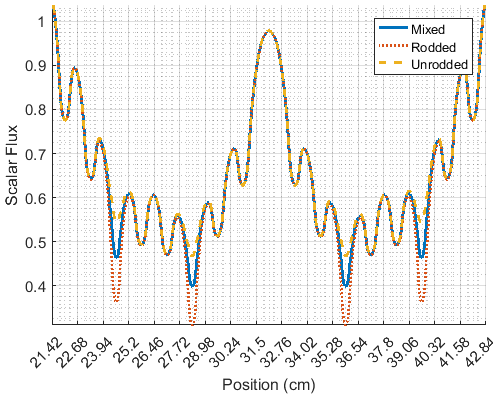
\includegraphics[width=0.7\textwidth]{1dmoc-50mix-fixedscat-scalflux7.png}
    \caption{Group 7 scalar flux comparisons for a fixed fission and scattering source calculation}\label{f:1dmoc-fixed-50-scalflux7}
\end{figure}

Figure \ref{f:1dmoc-fixed-50-angflux} shows the right-going angular flux in groups 1 (fast) and group 7 (thermal).  The group 7 angular flux behaves similarly to the group 7 scalar flux in that the effects are localized around each rod.  The three different angular flux shapes are still somewhat different at the edge of the neighboring pin cell, but have pretty much converged upon reaching the clad and fuel.  The reason for this is that the mean free path of thermal neutrons is small.  The total group 7 cross-section in the moderator is about 2.65 cm$^{-1}$, which corresponds to a mean free path of about 0.38 cm, which is less than one third of the pin pitch for a typical PWR.  Because of this, the differences between the rodded and unrodded cases are washed out quickly if the source distribution is kept the same between the two calculations.

\begin{figure}[H]
    \centering
    \subfigure[Group 1]{
        \centering
        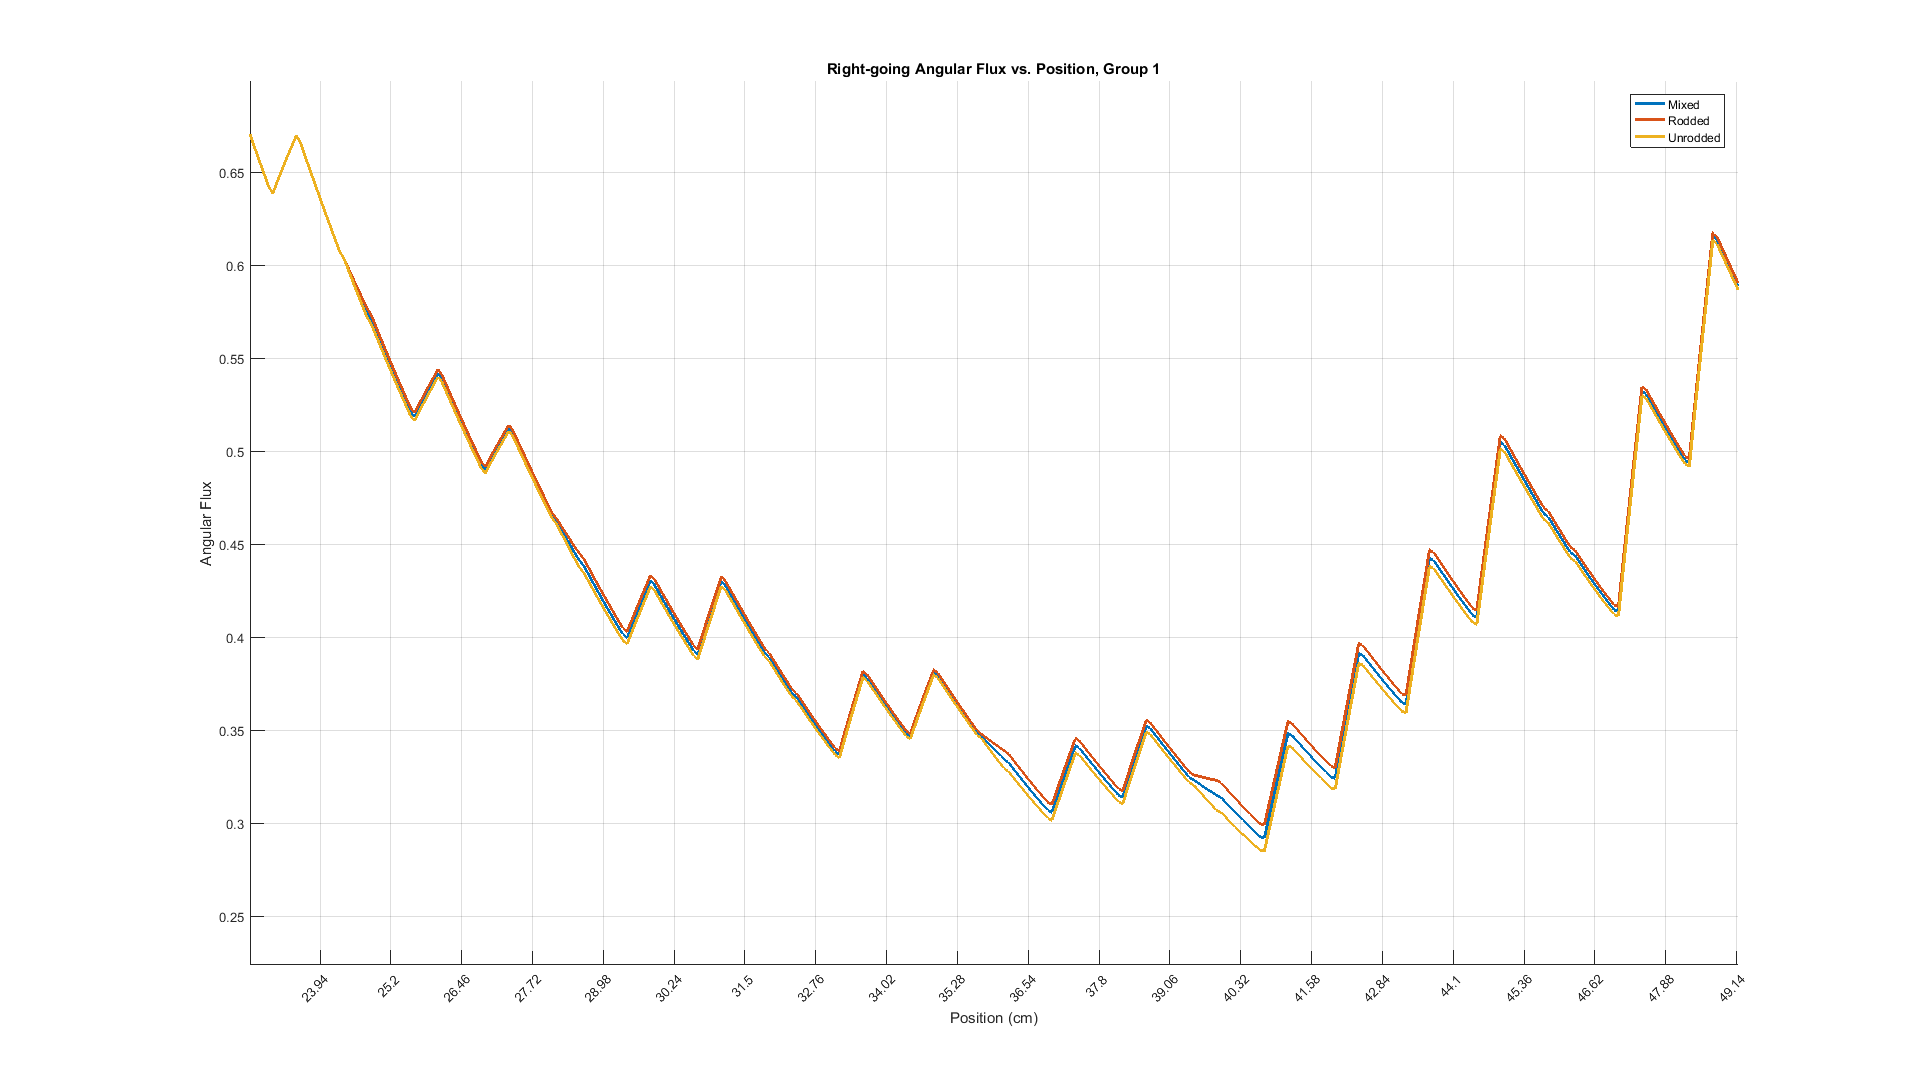
\includegraphics[width=0.6\textwidth]{1dmoc-50mix-fixedscat-angflux1.png}
        \label{f:1dmoc-fixed-50-angflux1}
    }
    ~
    \subfigure[Group 7]{
        \centering
        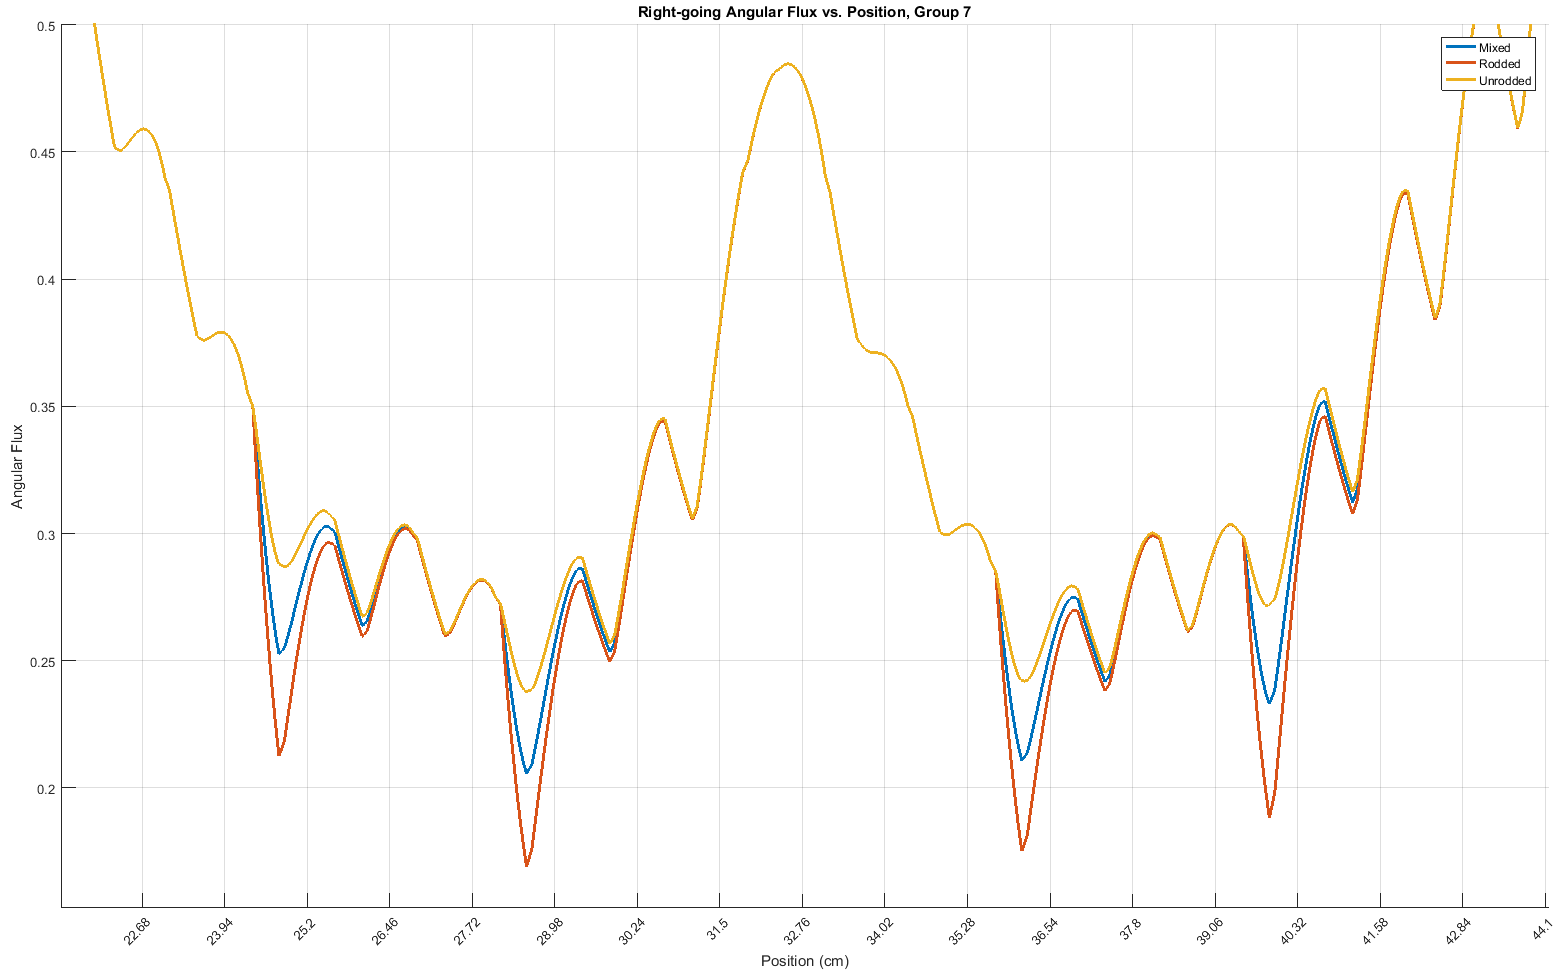
\includegraphics[width=0.6\textwidth]{1dmoc-50mix-fixedscat-angflux7.png}
        \label{f:1dmoc-fixed-50-angflux7}
    }
    \caption{Angular flux comparisons for a fixed fission and scattering source calculation}\label{f:1dmoc-fixed-50-angflux}
\end{figure}

The same cannot be said for the fast flux.  The mean free path of the fast flux is about 6.3 cm, which is the width of five pin cells.  Thus, it can be seen that each of the control rods after the first builds on the effects of the previous control rod.  While the fast flux does not have a significant impact on the fission source distribution, it does impact the scattering source distribution, which is not shown in these results.

\paragraph{Fixed Fission Source}

\begin{figure}[H]
    \centering
    \subfigure[25\% Mixture]{
        \centering
        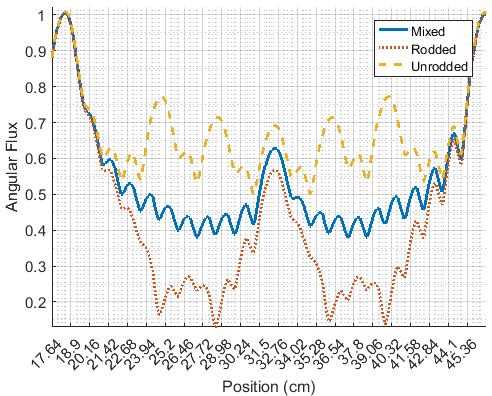
\includegraphics[width=0.45\textwidth]{1dmoc-25mix-angflux7.png}
        \label{f:1dmoc-25-angflux7}
    }
    \hfill
    \subfigure[50\% Mixture]{
        \centering
        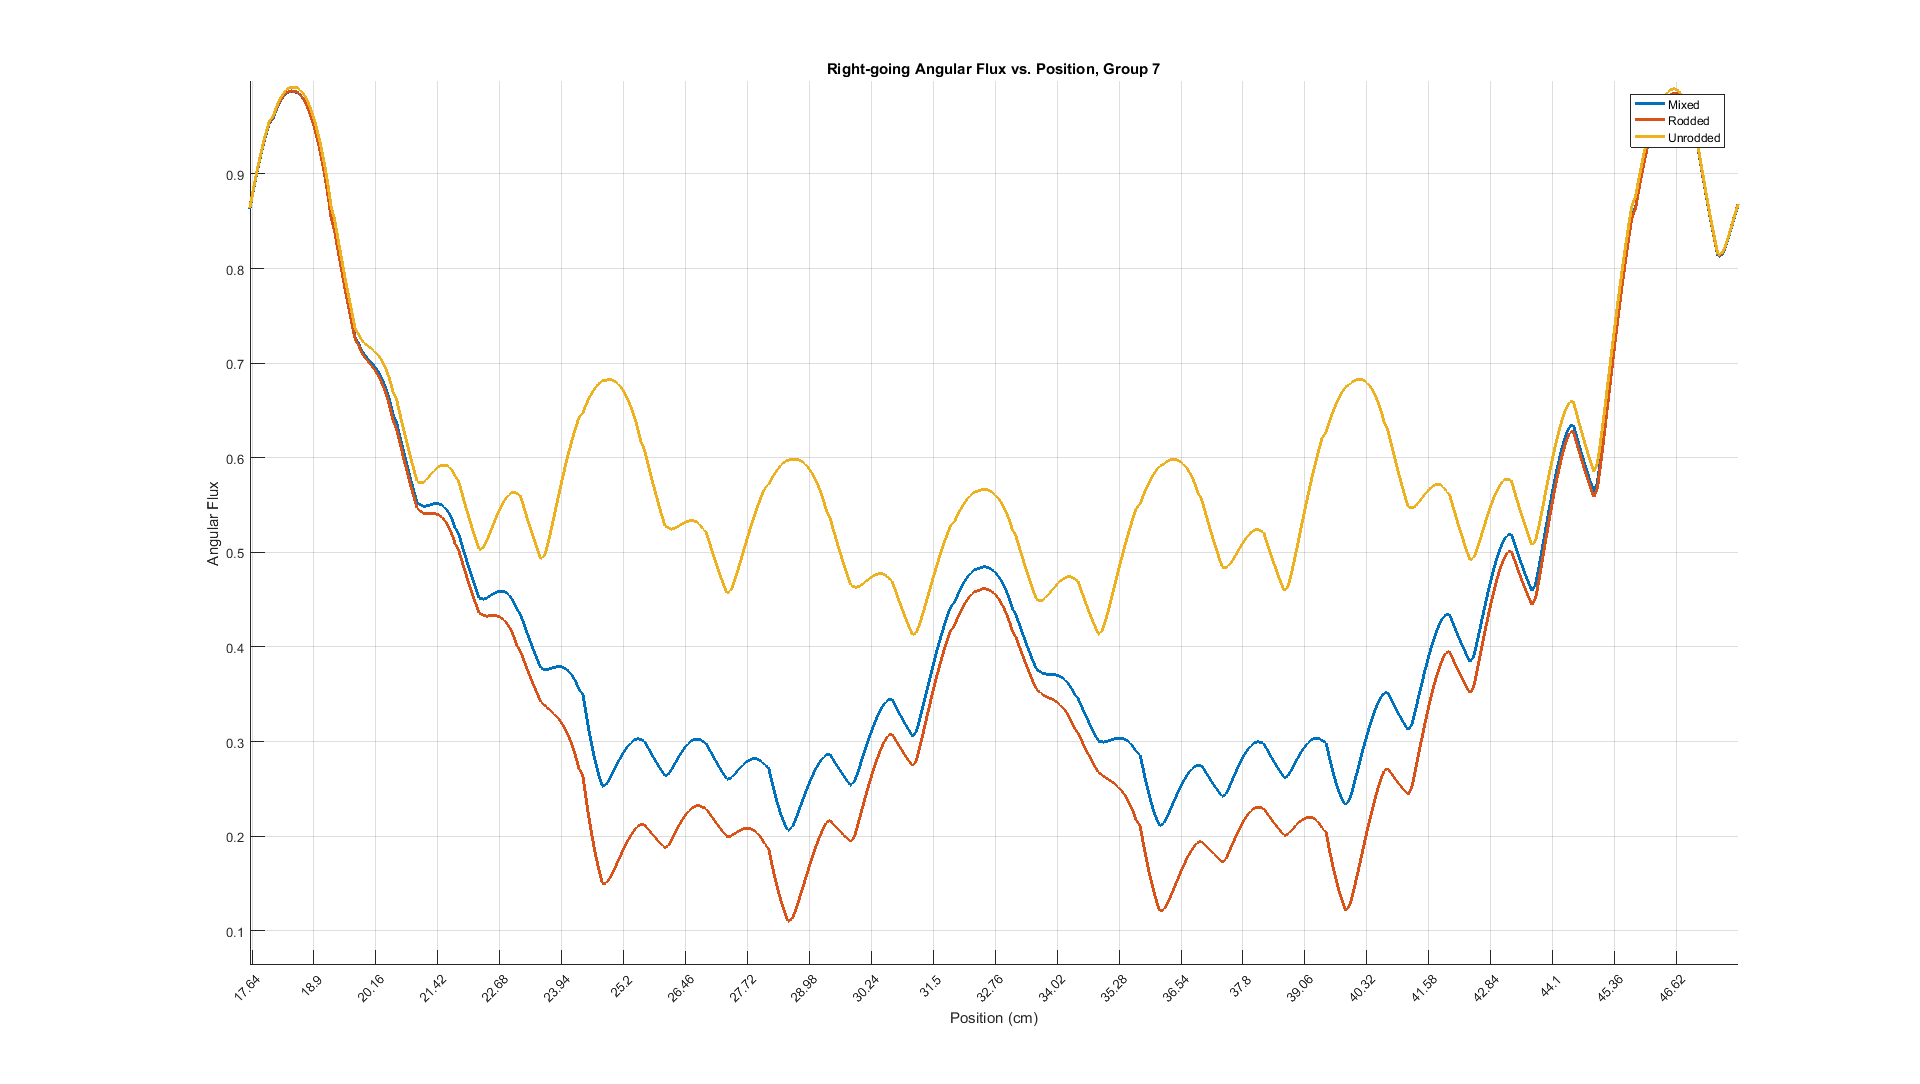
\includegraphics[width=0.45\textwidth]{1dmoc-50mix-angflux7.png}
        \label{f:1dmoc-50-angflux7}
    }
    ~
    \subfigure[75\% Mixture]{
        \centering
        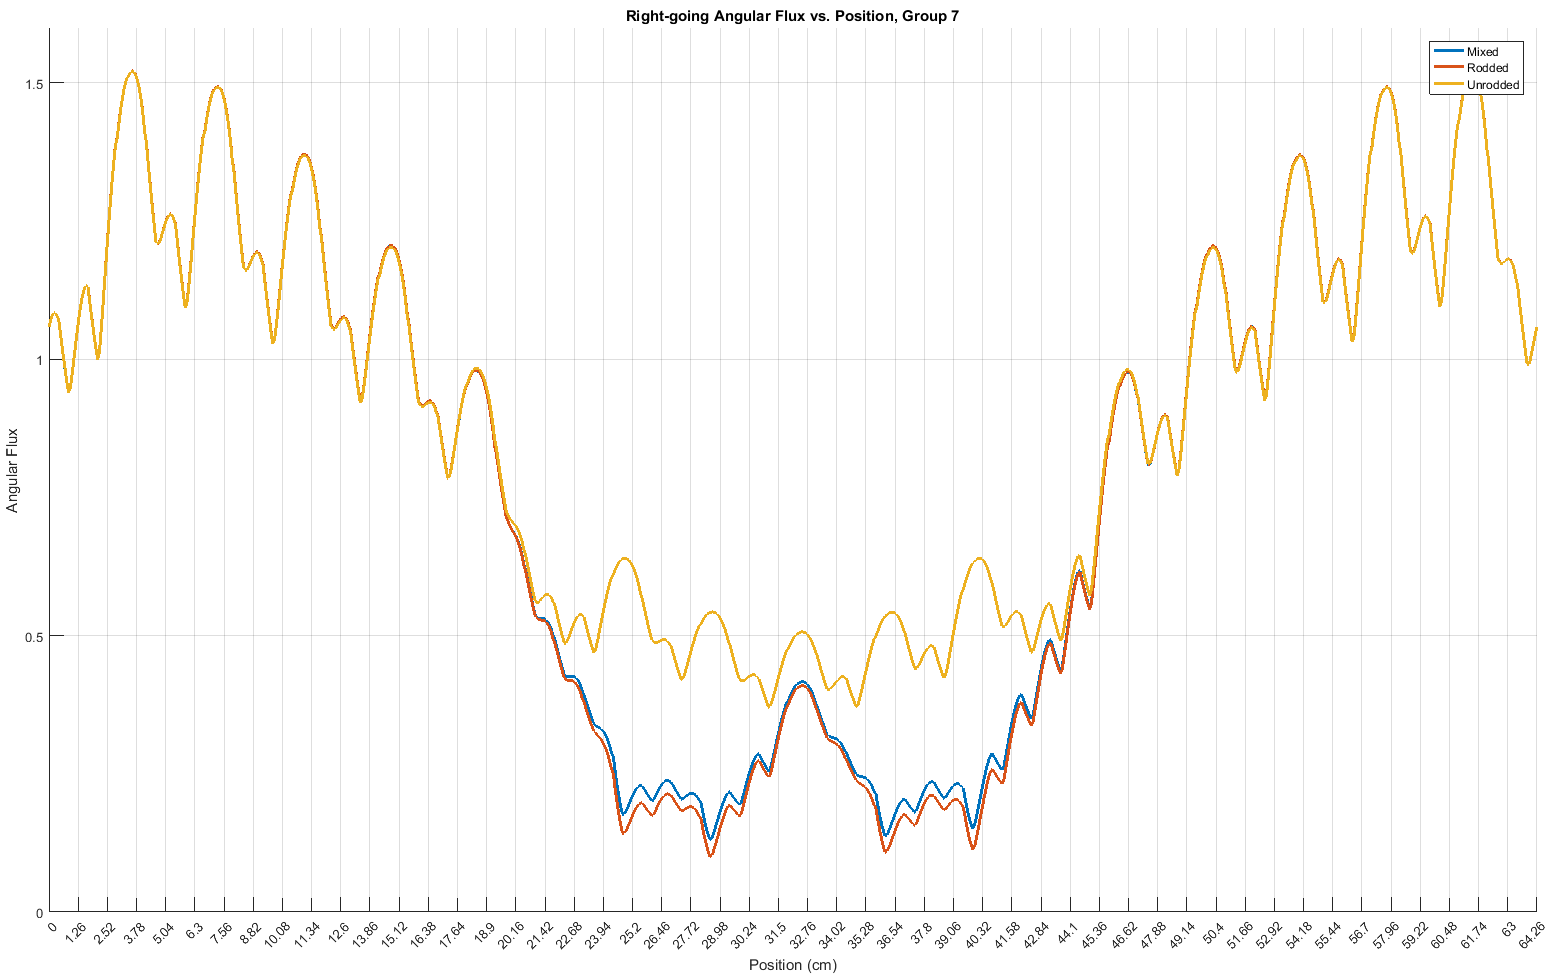
\includegraphics[width=0.45\textwidth]{1dmoc-75mix-angflux7.png}
        \label{f:1dmoc-75-angflux7}
    }
    \caption{Group 7 angular flux comparisons for 25\% and 75\% mixtures}\label{f:1dmoc-angflux7}
\end{figure}

The second set of calculations that was performed used a fixed fission source, but allowed the scattering source to fully converge for each calculation.  As in the previous section, an eigenvalue calculation was completed using partially rodded cross-sections.  This was done for 25\%, 50\%, and 75\% rodded cases.  For each case, a fixed fission source calculation was done with the fully rodded and fully unrodded cross-sections.  This time, multiple iterations were allowed for each material to converge the scattering source.  This allows us to see the effects of the rod on the scattering source distribution without worrying about changes in the eigenvalue and fission source distribution.

\begin{figure}[H]
    \centering
    \subfigure[25\% Mixture]{
        \centering
        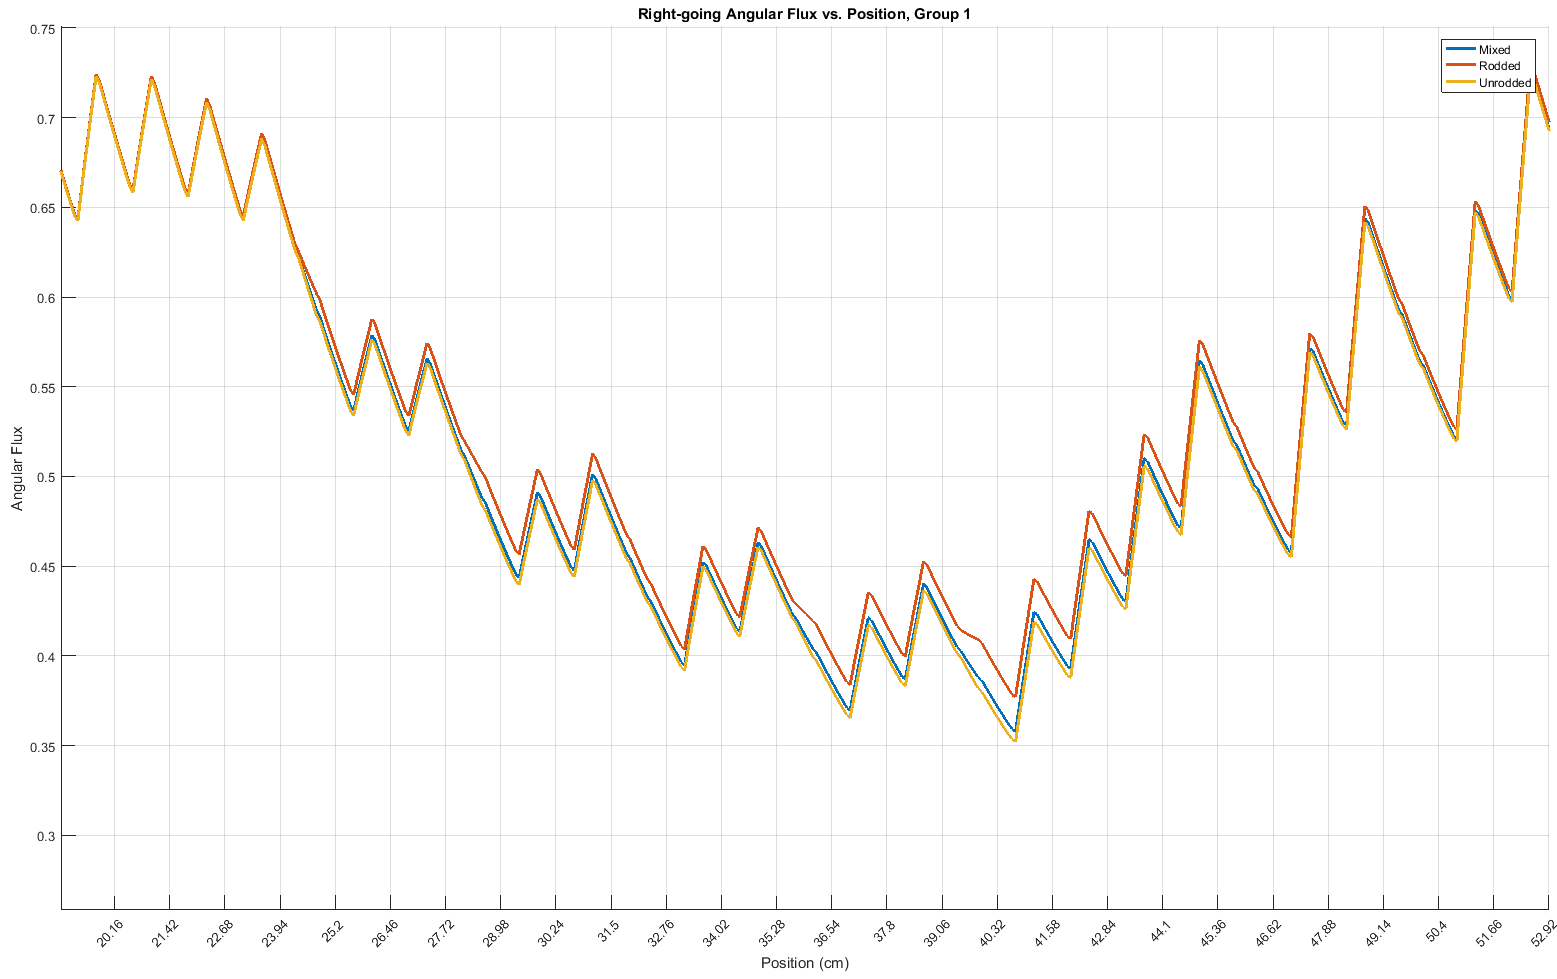
\includegraphics[width=0.45\textwidth]{1dmoc-25mix-angflux1.png}
        \label{f:1dmoc-25-angflux1}
    }
    \hfill
    \subfigure[50\% Mixture]{
        \centering
        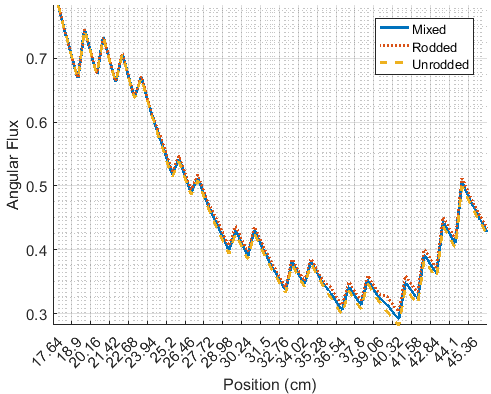
\includegraphics[width=0.45\textwidth]{1dmoc-50mix-angflux1.png}
        \label{f:1dmoc-50-angflux1}
    }
    ~
    \subfigure[75\% Mixture]{
        \centering
        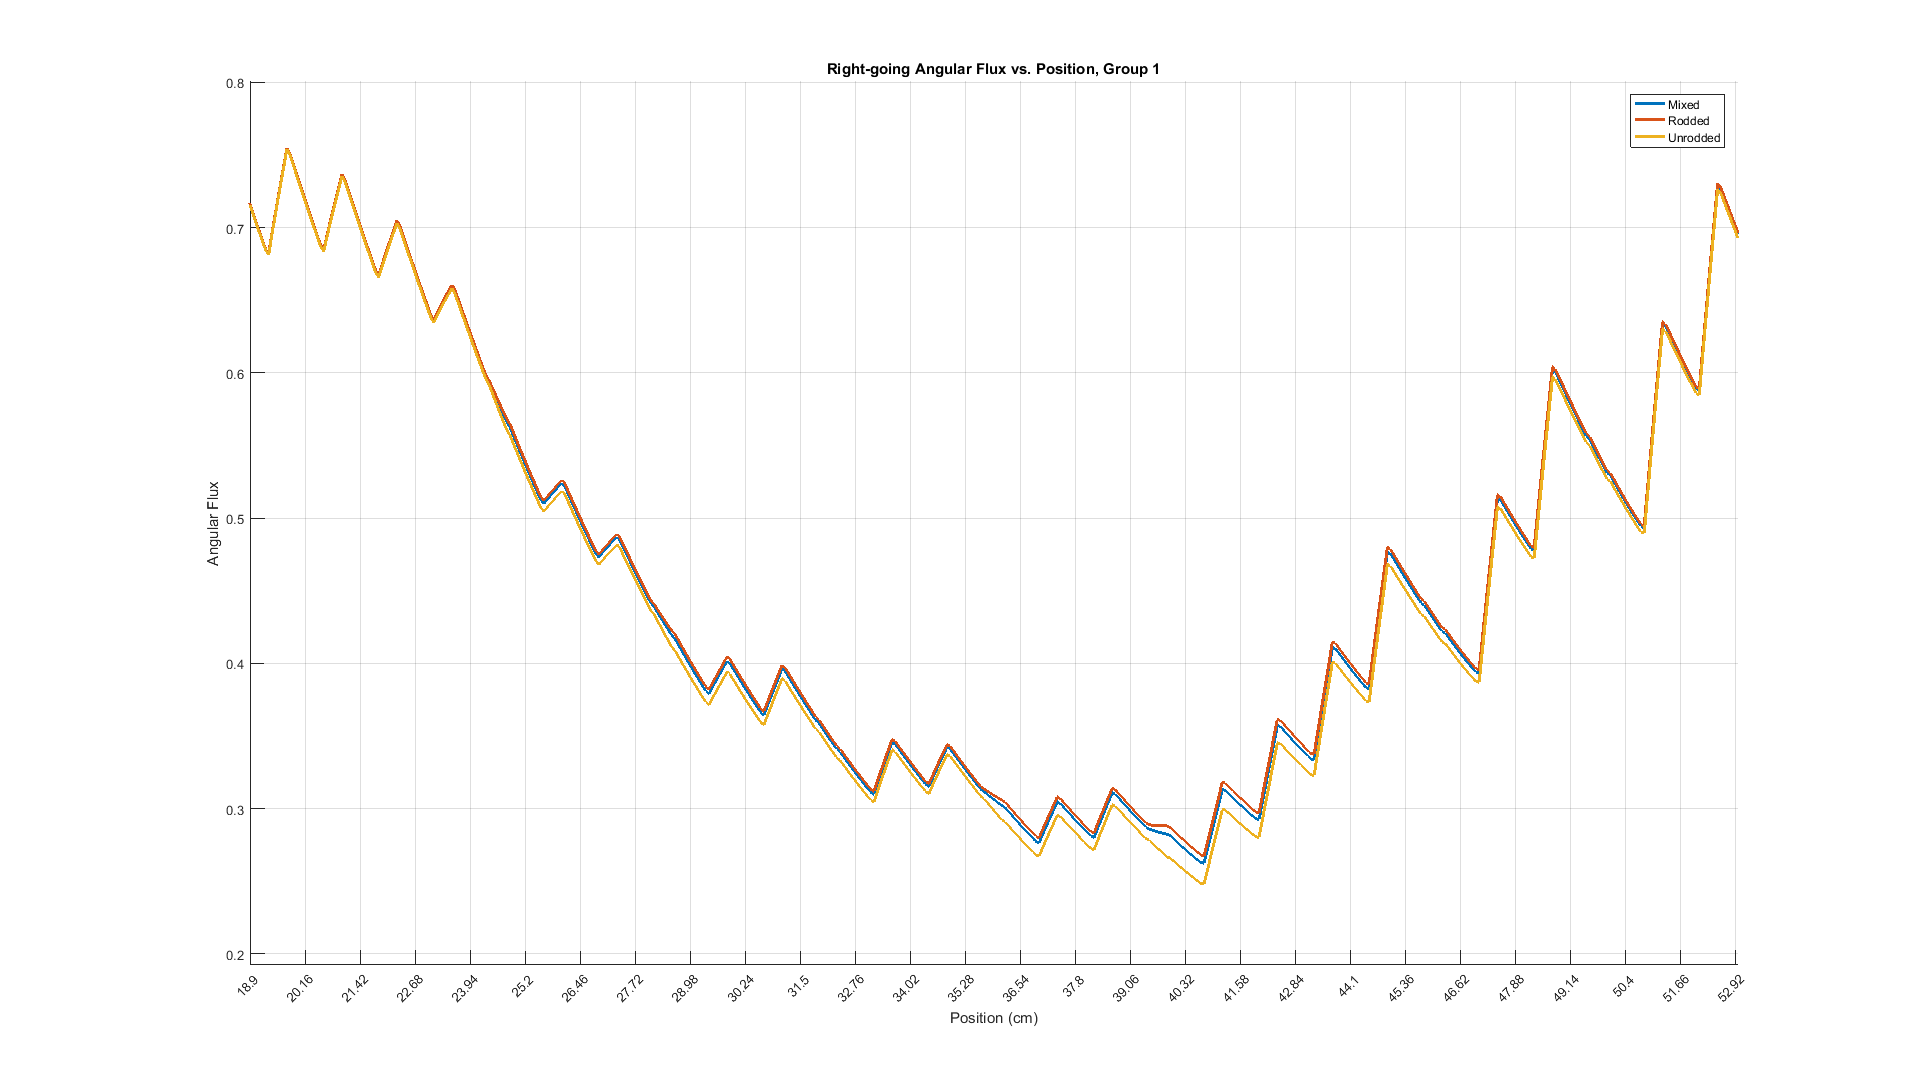
\includegraphics[width=0.45\textwidth]{1dmoc-75mix-angflux1.png}
        \label{f:1dmoc-75-angflux1}
    }
    \caption{Group 1 angular flux comparisons for 25\% and 75\% mixtures}\label{f:1dmoc-angflux1}
\end{figure}


Figure \ref{f:1dmoc-angflux7} shows the group 7 angular flux comparisons for each of the three mixtures.  We immediately see that for each of them, the angular flux for the mixture is closer to the rodded result than the unrodded result than what might be expected based on the volume fraction of the rod.  For example, comparing Figures \ref{f:1dmoc-50-angflux7} and \ref{f:1dmoc-fixed-50-angflux7} shows that the angular flux is much closer to the rodded solution than when the scattering source was fixed, despite the small mean free path of thermal neutrons.  Figure \ref{f:1dmoc-angflux1} shows the same comparisons for the group 1 angular flux.  While the difference in magnitude between each of the three cases is small for any mixture, the long mean free path means that these differences get spread out over a larger area.  This changes the shape of the scattering source for the thermal groups, which then has a more widespread effect on the the scalar flux distribution.  It should be noted as well that all angular flux plots shown here are for the flattest polar angle.  Since the steeper angles travel through more material in each region, the differences between them go away more quickly.  Thus, the angle shown in these plots is the one having the largest impact on the solution.

\subsection{Subray MOC Description}